\section{Day 15: Compactness (Oct. 22, 2024)}
Outfit of the day: balatro theme
\begin{figure}[h]
    \centering
    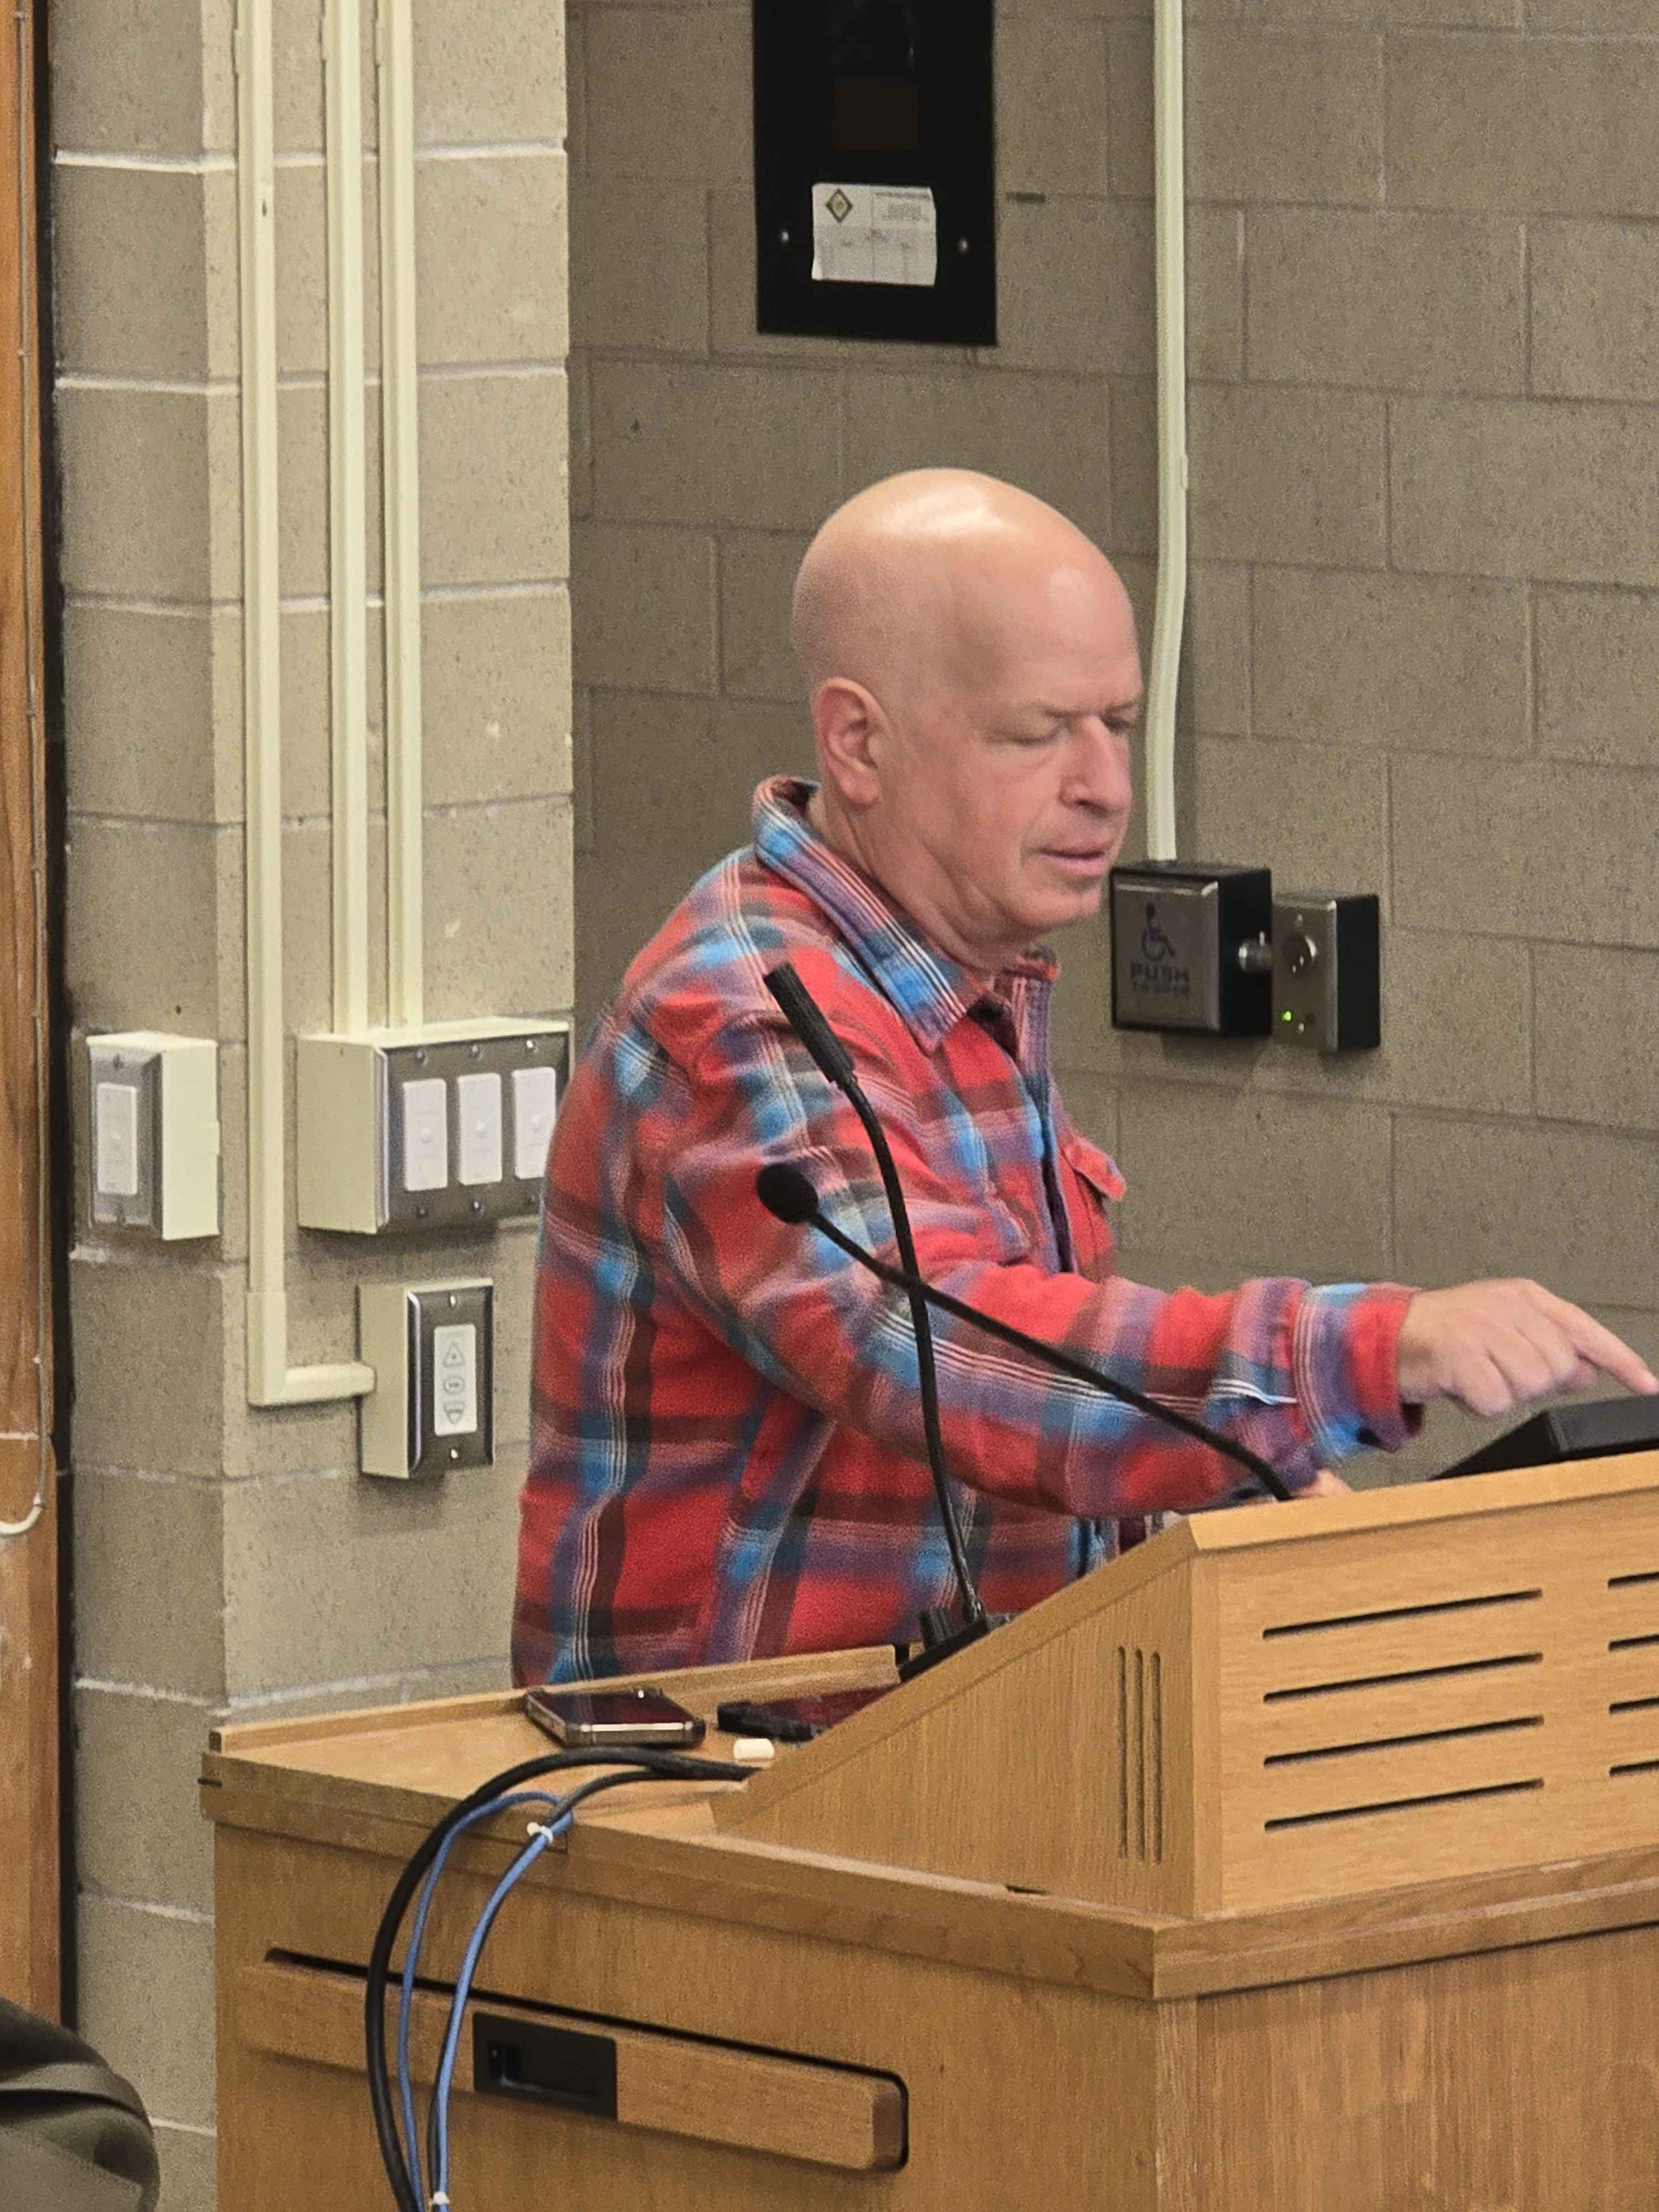
\includegraphics[scale=0.1]{MAT327 Notes/Dror Shirts/dror day 15 shirt.jpg}
\end{figure}

\noindent Our goal for today is to imitate the proof that, on a compact set, every continuous function $F : X \to \RR$ is bounded. Start by observing that every continuous function is "locally bounded" (read: $\eps-\delta$), where \textit{locally} means that every point has a neighborhood in which $f$ is bounded\footnote{In general, \textit{locally} [topo property] means that said property holds in some open neighborhood about every point. Something on basic sets maybe, check lance}.
\medskip\newline
To prove this, given a point $x \in X$, we have that $U = f^{-1}((f(x) - 1, f(x) + 1))$ be a neighborhood of $x$ on which $f$ is bounded. Compactness is a property of spaces that intuitively means a local property is true globally as well. A topological space $X$ is called \textit{compact} if it has a finite cover by open sets.
\begin{definition}
    A \textit{cover} of a set $X$ is a collection $A$ of subsets of $X$ such that $\bigcup_{A \in U} A = X$. If all the sets in $A$ are open, we say that $U$ is an open cover.
\end{definition}
\noindent We say that a topological space $X$ is called compact if every open cover of $X$ has a finite subcovering.

\newpage
\begin{simplethm}
    A continuous function on a compact space is bounded. Namely, if $X$ is compact and $f : X \to \RR$ is continuous, then there exists $M > 0$ such that, for all $x \in X$, $\abs{f(x)} < M$.
\end{simplethm}
\noindent Let $\SO = \{U_x = f^{-1}((f(x) - 1, f(x) + 1)) \mid x \in X\}$ is an open cover of $X$, as each $U_x$ is open, and all $x \in X$ are in $U_x$, we see that $\SO$ covers $X$; by compactness, there exists a finite subcover $U_{x_1}, \dots, U_{x_n}$; then we may take a maximum of the bounds on each $U_{x_i}$, i.e. $M = \max\{\abs{f(x_1)} + 1, \dots, \abs{f(x_n)} + 1\}$ to see that $f$ is bounded above by $M$. \qed
\begin{simplethm}
    $[0, 1]$ is compact.
\end{simplethm}
\noindent Let $\SO$ be an open cover of $[0, 1]$, and set $G = \{ g \in [0, 1] \mid [0, g] \text{ covered by finitely many } U \\ \in \SO\}$. Start by observing that $G$ is not empty because $0 \in G$, and $G \in [0, 1]$ so it is bounded. Let $m = \sup G$; we want to prove that $1 \in G$. To start, $m > 0$; indeed, pick $U \in \SO$ such that $0 \in U$, which is possible because the cover covers the entire of $[0, 1]$. $U$ is open, so for some $\eps > 0$, $[0, \eps) \in U$, so $U$ covers $[0, \frac{\eps}{2}]$, meaning $\frac{\eps}{2} \in G$ and so $m \geq \frac{\eps}{2} > 0$.
\medskip\newline
We now show that $m = 1$. Assume not, i.e. $0 < m < 1$. Let $U \in \SO$ be a neighborhood of $m$; then $(m-\eps, m+\eps) \in U$ for $\eps > 0$, meaning $[m-\frac{\eps}{2}, m+\frac{\eps}{2}] \in U$; taking a finite subcover of $[0, m']$ (for some $m - \frac{\eps}{2} < m' < m$, which is necessarily in $G$, otherwise $m$ is not the supremum) and appending $[m - \frac{\eps}{2}, m + \frac{\eps}{2}]$, we see that $[0, m + \frac{\eps}{2}] \in G$, meaning $\sup G \neq m$, which is a contradiction. Thus, $m = 1$.
\medskip\newline
Indeed, find $U \in \SO$ such that $1 \in U$; let $\eps > 0$ such that $(1 - \eps, 1] \in U$. Find $g \in G$ such that $1 - \eps < g \leq 1$. Then $[0, g]$ has a finite cover, and $[0, g] \cup U = [0, g] \cup (1 - \eps, 1] = [0, 1]$, which has a finite cover as well. \qed
\begin{simplethm}
    A closed subset $C$ of a compact set $X$ is compact.
\end{simplethm}
\noindent Picture proof was given, but just use Heine-Borel... (closed and bounded).